%!TEX root = ../thesis.tex

\chapter{Постановка задачі дослідження та огляд існуючих методів її розв'язання}
\label{chap:review}  %% відмічайте кожен розділ певною міткою -- на неї наприкінці необхідно посилатись

\section{Метод Marked Point Processes}

Одним з сучасних методів визначення кратерів на супутникових
знімках є робота~\cite{mpp2022}. У статті представлено
стохастичний підхід, заснований на процесах маркованих
точок (MPP) для автоматичного виявлення бомбових
воронок на аерофотознімках воєнного часу. Метод
використовує виявлені воронки для створення карти
впливу, яка класифікує території як потенційно забруднені
або незабруднені на основі ймовірності наявності
нерозірваних боєприпасів. Підхід було протестовано
на знімках з Нижньої Саксонії, Зальцбурга та Італії,
причому оцінювання проводилося як на основі об'єктів,
так і на основі пікселів. Експерименти були зосереджені
на аналізі моделі, впливу різних параметрів і порівнянні
з об'єктним детектором на основі глибокого навчання.

При аналізі моделі порівнювалися результати, отримані
при використанні кола та еліпса в якості об'єктної моделі.
Було виявлено, що при використанні еліпса дещо підвищується
повнота, але знижується точність, що робить
модель кола більш стабільною.

F1 score -- це показник, який використовується в статистичному аналізі для
оцінки точності тесту на бінарну класифікацію. Це середнє гармонійне значення
точності та повноти, що забезпечує баланс між цими двома показниками. Це робить
його особливо корисним в ситуаціях, коли потрібно знайти баланс між точністю
(точністю позитивних прогнозів) і повнотою (здатністю знайти всі позитивні
приклади).

Дослідження також оцінило важливість різних енергетичних доданків у моделі,
показавши, що виключення певних доданків призводило
до збільшення кількості хибних спрацьовувань і зменшення
показника F1. Результати продемонстрували ефективність
запропонованої моделі для точного виявлення бомбових кратерів.

У дослідженні також вивчався вплив використання надлишкової
інформації зображення шляхом об'єднання результатів виявлення
з декількох зображень, що покривають одну і ту ж ділянку.
Результати показали значне покращення показника F1 при
об'єднанні результатів виявлення, що вказує на потенціал
використання декількох зображень для підвищення точності
виявлення. Крім того, дослідження було зосереджено на
оптимізації точності результатів, що має вирішальне
значення для запропонованого сценарію застосування,
шляхом варіювання параметрів для досягнення більш високої
точності за рахунок повноти.

Порівняння підходу MPP з детектором об'єктів на основі
глибокого навчання показало, що модель глибокого
навчання перевершує підхід MPP в сценаріях з достатньою
кількістю маркованих навчальних даних. Однак у сценаріях
з обмеженою кількістю мічених даних або взагалі без них
підхід MPP показав кращі результати. Дослідження підкреслило
перевагу підходу на основі моделей у сценаріях, де навчальних
даних недостатньо або вони взагалі відсутні, що дозволяє
уникнути необхідності великого ручного маркування.

Загалом, результати дослідження продемонстрували ефективність
підходу MPP в автоматичному виявленні вирв від бомб на
аерофотознімках воєнного часу. Метод показав багатообіцяючі
результати у позначенні зон впливу з високою точністю.
У той же час, метод не найкращим чином придатний для точного
виявлення кратерів на знімках.

\section{Підхід з використанням CNN}

Згорткові нейронні мережі (CNN)~\cite{oshea2015} -- це тип штучних
нейронних мереж,
який зазвичай використовується для аналізу візуальних даних,
таких як зображення. Вони отримали свою назву
через використання операції згортки, яка є основною
для виявлення візуальних шаблонів або функцій у вхідних даних.
Одна з ключових особливостей CNN -- це використання шарів згортки
та пулінгу, які допомагають зменшити кількість параметрів у мережі
і забезпечують роботу з об'єктами різних розмірів у вхідних даних.

Згорткові нейронні мережі широко застосовуються в різних задачах
обробки зображень, таких як розпізнавання об'єктів, класифікація
зображень, виявлення облич, а також у задачах комп'ютерного зору.
Їхній успіх полягає в здатності автоматично вивчати корисні функції
зображень з великою кількістю даних для тренування, що робить їх
ефективним інструментом у багатьох сферах, включаючи медицину,
автомобільну промисловість та аналітику зображень.

Робота~\cite{clermont2019} використовує CNN для розв'язання задачі
бінарної класифікації, тобто по зображенню визначає, чи є на ньому кратер,
чи це фонове зображення.

На рисунку~\ref{cnn_paper_arch} зображена кінцева архітектура мережі. Як видно,
до готового екстрактора підключені два повнозв'язних шари, які потім підключені
до ще одного softmax шару. Під час тренування, оновлюються ваги останніх двох
шарів попередньо навченої мережі (Block 8 і шар FC), а також шари, додані
авторами.

\begin{figure}[ht]
      \centering
      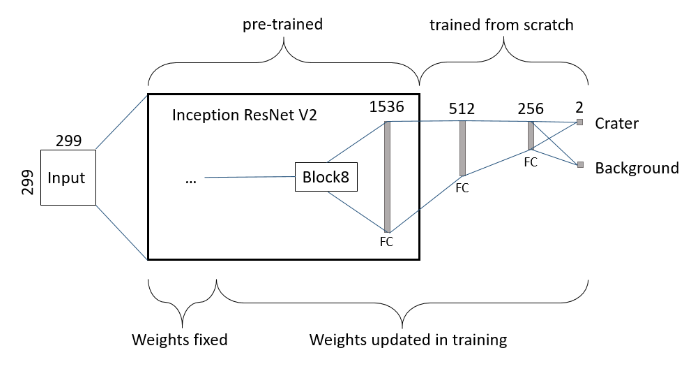
\includegraphics[scale=0.75]{Images/paper_arch.png}
      \caption{Архітектура мережі, запронованої у роботі~\cite{clermont2019}}
      \label{cnn_paper_arch}
\end{figure}

У статті представлено метод контрольованого виявлення вирв
від бомб на історичних аерофотознімках з використанням
згорткових нейронних мереж (CNN). Метою дослідження є
автоматичне виявлення кратерів від бомб на знімках часів
Другої світової війни для відстеження бомб, що не розірвалися,
які все ще становлять загрозу сьогодні. Метод складається з
двох основних етапів: вилучення кандидатів у кратери за
допомогою детектора блобів (від англ. blob, що в даному контексті
означає форму кратера) і класифікація цих кандидатів
як кратерів або фону за допомогою CNN. Підхід має
на меті покращити виявлення кратерів від бомб на
історичних знімках, що може бути складним завданням
через варіації зовнішнього вигляду кратерів та неточності
в довідкових анотаціях.

Експерименти, проведені в дослідженні, виявили цікаві
результати. Процес виділення кандидатів за допомогою
детектора блобів показав, що метод не може досягти необхідної
точності, вказуючи на те, що не всі еталонні кратери
були виділені як кандидати. Це може бути пов'язано з
обмеженнями обраних параметрів блоб-детектора, оскільки
деякі кратери на зображеннях не мали чіткого блобоподібного
вигляду. Крім того, порівняння з методом ковзного вікна
показало необхідність подальшої оптимізації параметрів
для покращення процесу виділення кандидатів.

З точки зору класифікації, експерименти продемонстрували
вплив ваги помилкових спрацьовувань на результати.
Використання ваги, що відповідає співвідношенню позитивних
і негативних вибірок, значно покращило показник F1,
що вказує на важливість балансування помилок класифікації.
Однак переносимість між наборами даних була не такою успішною:
CNN показала кращі результати на тому наборі даних,
на якому вона навчалась. Це свідчить про те,
що відмінності між наборами даних і неточності
в довідкових анотаціях можуть впливати на результати класифікації.

У дослідженні також вивчалося поєднання наборів
даних для покращення результатів класифікації. Хоча навчання
і тестування на комбінованому наборі даних не дало кращих
результатів порівняно з навчанням на окремих наборах даних,
необхідні подальші дослідження, щоб зрозуміти вплив відмінностей
у наборах даних на роботу CNN. Результати свідчать про те,
що CNN може мати труднощі з перенесенням знань між наборами
даних з різними характеристиками, що підкреслює необхідність
застосування методів адаптації до предметної області для
підвищення точності класифікації. Загалом, дослідження дає
цінну інформацію про виклики і можливості автоматизованого
виявлення вирв від бомб на історичних аерофотознімках за
допомогою CNN. В той же час, результати виявилась недостатньо
гарними для того, щоб назвати запропоновану архітектуру
точною та ефективною. Крім того, дана модель використовується
лише для класифікації зображень, а не для сегментації.

\section{Методи, засновані на статистичних індикаторах}

Роботи~\cite{mikava2023,shelestov2023} виявляють та аналізють пошкодження
територій за допомогою
індексу рослинності NDVI, при цьому інформація оцінюється
за певні часові інтервали.

Дослідження фокусується на виявленні типових пошкоджень,
таких як воронки від обстрілів і вибухів, вигорілі поля
та сліди військової техніки. Оцінці втрат від конфлікту в
Україні присвячено багато робіт, в яких застосовуються
різні методи -- від виявлення воронок до оцінки пошкоджень
міських територій. Супутникові дані, зокрема місії
Sentinel-2, відіграють вирішальну роль у цьому аналізі.

Методологія передбачає розрахунок
індексу NDVI та аналіз спектральних каналів для виявлення
пошкоджених сільськогосподарських угідь. У дослідженні
оцінка поділяється на двотижневі періоди і порівнюються
значення NDVI до і після конкретних подій для точного
моніторингу пошкоджень. Результати показують, що метод,
заснований на відносній різниці у значеннях NDVI, дозволяє
виявити значно більшу кількість пошкоджених полів порівняно
з візуальною оцінкою.

Валідація методу включала візуальну перевірку вибраних
ділянок і порівняння з оперативними даними ACLED.
Дослідження успішно виявило пошкоджені поля в Донецькій області,
що відповідає офіційним повідомленням про обстріляні території.
Метод виявився ефективним у виявленні пошкоджень, особливо
в районах, близьких до зон активних бойових дій.

До переваг запропонованого методу виявлення пошкоджень
сільськогосподарських угідь з використанням супутникових
даних та вегетаційного індексу NDVI можна віднести наступні:

\begin{itemize}

      \item Об'єктивна оцінка: Метод забезпечує
            об'єктивну оцінку пошкоджень на основі
            кількісних даних, що зменшує ймовірність
            упередженості в оцінках.
      \item Масштабованість: Метод можна
            застосовувати в різних масштабах,
            від окремих полів до великих регіонів,
            що робить його універсальним для різних рівнів аналізу.

\end{itemize}

До недоліків запропонованого методу можна віднести:

\begin{itemize}

      \item Сезонна мінливість: Сезонні
            зміни рослинності та умов навколишнього
            середовища можуть впливати на значення NDVI,
            що вимагає ретельного розгляду і потенційно
            впливає на точність виявлення пошкоджень.
      \item Верифікація: Хоча метод забезпечує
            автоматизоване виявлення пошкоджень,
            для підтвердження точності результатів може
            знадобитися ручна перевірка, що додає додатковий
            етап до процесу.
      \item Доступність даних: Ефективність
            методу залежить від наявності високоякісних
            супутникових даних, які не завжди можуть
            бути постійно доступними або актуальними в
            регіонах, що постраждали від конфлікту.

\end{itemize}

Загалом, хоча запропонований метод пропонує значні переваги
в оцінці збитків, завданих сільськогосподарським угіддям,
важливо враховувати ці обмеження, щоб забезпечити точність
і достовірність результатів.

Ще одним прикладом застосування індексу NDVI є робота~\cite{deininger2023}, у якій
NDVI використовується для оцінки врожайності полів озимих зернових. Результати
показують, що даний метод є ефективним для оцінки пошкоджень такого типу.

Робота~\cite{kussul2023} представляє комплексну методологію автоматичної ідентифікації
сільськогосподарських територій, пошкоджених діями у воєнний
час, з використанням супутникових даних Sentinel-2.

Методологія, описана в статті, передбачає використання
спектральних смуг з роздільною здатністю 10 м та
індексів рослинності з даних Sentinel-2,
а також статистичних показників за певний проміжок часу,
як вхідних даних для класифікатора Random forest.
Алгоритм ефективно визначає пошкоджені поля з високою
точністю близько 0.85. Потім використовується підхід
виявлення аномалій для окреслення пошкоджень в межах
полів шляхом поєднання спектральних смуг та індексів.

У статті~\cite{kussul2023} використані наступні статистичні показники:

\begin{itemize}

      \item NDVI -- це загальновизнаний вегетаційний індекс, який вимірює стан і щільність
            рослинності. У дослідженні NDVI використовується для виявлення аномалій у
            рослинному покриві, особливо у відповідь на пошкодження, спричинені військовою
            діяльністю.
      \item EVI -- це ще один вегетаційний індекс, який використовується для оцінки
            здоров'я та щільності рослинності. У цьому дослідженні EVI розглядається разом
            з NDVI для оцінки впливу пошкоджень на сільськогосподарські поля.
      \item AVI -- це вегетаційний індекс, який включає в себе певні спектральні діапазони
            для оцінки здоров'я та життєздатності рослинності. Він використовується в
            дослідженні для доповнення аналізу пошкоджень на сільськогосподарських полях.
      \item GCI -- це вегетаційний індекс, який фокусується на вмісті хлорофілу в
            рослинності. У дослідженні GCI використовується для виявлення аномалій у
            рослинному покриві та оцінки пошкоджень сільськогосподарських полів.

\end{itemize}

Дослідження, проведене протягом 22
двотижневих періодів у 2022 році, виявило
близько 500 тисяч гектарів орних земель у
10 регіонах України, які були пошкоджені. Результати методології
демонструють ефективність автоматизованого супутникового
моніторингу для оцінки впливу військових дій на сільське
господарство.

Ще одним індексом, який можна використати для визначення пошкоджень,
є NDWI -- індекс дистанційного зондування, який використовується
для визначення та моніторингу наявності водних об'єктів,
вмісту води в рослинності та змін у вмісті води в рослинному покриві~\cite{kussul20232}.
Підхід було застосовано на тестовій ділянці площею 8 800
га в Донецькій області. Використовуючи знімки PlanetScope
з роздільною здатністю 3 метри, автори змогли виявити 202 гектари
кратерів, що становить 63\% від виявлених на знімках SkySat.
На знімках Sentinel-2 з роздільною здатністю 10 метрів автори
виявили 165 гектарів кратерів, або 51\% від тих, що були
виявлені на знімках SkySat.

\section{Постановка задачі}

Основною задачею є розробка автоматизованого методу точної
сегментації та ідентифікації кратерів від вибухів бомб на супутникових
знімках. Цей метод спрямований на покращення виявлення,
моніторингу та аналізу наслідків вибухів бомб у зонах
конфліктів для гуманітарних та екологічних цілей.
Кратер -- це кругла або майже кругла заглибина,
що утворилася на поверхні землі внаслідок падіння та
вибуху бомби. Кратери зазвичай мають такі характеристики:
переважно круглу або еліптичну форму, підняті краї по
периметру, часто зі зміщеним ґрунтом або уламками,
помітну глибину порівняно з навколишньою місцевістю
а також виразні відмінності в текстурі всередині кратера
і в безпосередній близькості від нього, зумовлені вибуховою хвилею від вибуху.

Вхідні дані для цієї задачі складаються зі знімку та маски. Методологія включає в себе
декілька кроків. Спочатку треба підготувати датасет, фрагментуючі вхідні дані, для
отримання достатньої кількості навчального та тестового матеріалу. Наступним кроком
є імплементація моделей машинного навчання, навчання їх на тестовому датасеті
та отримання відповідних метрик, за якими потім буде проводитися
порівняльний аналіз моделей.

Метрики моделі включають точність, повноту, IoU та F1. За даними метриками
можна точно визначити моделі, які краще справляються з розв'язанням
задачі сегментації кратерів на супутникових знімках.

\section*{Висновки до розділу 1}

Отже, у даному розділі було проведено огляд існуючих методів
розв'язання задачі дослідження та формалізовано задачу
сегментації кратерів на супутникових знімках.
У приведених роботах використовувалися різні підходи, а саме MPP, CNN, та
методи, засновані на використанні статистичних показників.
MPP показав свою ефективність у розв'язуванні цієї задачі, особливо
за умов, коли немає розміченої маски, або коли даних недостатньо для
тренування більш складної CNN моделі. Методи, засновані
на статистичних показниках теж потребують менше даних за CNN,
але потрібні знімки, розподілені у часі, що може ускладнити успішне використання
цього методу.
У той же час, якщо даних достатньо,
то CNN дає більш точні результати.

У ході формалізації завдання було дано визначення поняттю кратера,
описані вхідні дані, кроки методології та метрики, за якими будуть
порівнюватися моделі машинного навчання.